\documentclass{beamer}
\usepackage[utf8x]{inputenc}

% For algorithms
\usepackage{algorithm}
\usepackage{algorithmic}
\usepackage{natbib}


\usetheme{Berlin}
\usecolortheme[RGB={0,150,150}]{structure}
\setbeamertemplate{navigation symbols}{}


%%%%% Comments, Todos, etc %%%%%

\newcommand{\fix}{\marginpar{FIX}}
\newcommand{\new}{\marginpar{NEW}}
\newcommand{\cmt}[1]{\textcolor{red}{#1}}
\newcommand{\todo}[1]{\textcolor{cyan}{#1}}

%%%% General, Operators %%%%
\DeclareMathOperator*{\argmin}{arg\,min}
\DeclareMathOperator*{\argmax}{arg\,max}
\newcommand{\trans}{\top} %matrix transpose

\newcommand{\code}[1]{\texttt{#1}}

%%%% Set Theory %%%%%%%
\newcommand{\card}[1]{\vert #1 \vert} %cardinality
\newcommand{\Reals}{\mathbb{R}}
\newcommand{\Nats}{\mathbb{N}}

%%%% Complexity %%%%%%%
\newcommand{\BigO}{\mathcal{O}} %Big-O-notation


%%% Probability theory %%%%%
\newcommand{\Prob}{\mathbb{P}}

\newcommand{\Expect}{\mathbb{E}}
\newcommand{\Var}{\mathbb{V}}
\newcommand{\Cov}{\textrm{Cov}}
\newcommand{\Corr}{\textrm{Corr}}

\newcommand{\indep}{\protect\mathpalette{\protect\independenT}{\perp}}\def\independenT#1#2{\mathrel{\rlap{$#1#2$}\mkern2mu{#1#2}}} %alternative: \!\perp\!\!\!\perp
\newcommand{\dep}{\not\indep}

\newcommand{\DistrDist}[2]{\mathcal{D}(#1,#2)} %General distance between distributions
\newcommand{\distTV}[2]{|#1,#2|_\textrm{TV}} %Total Variation distance

\newcommand{\Rv}{x} % random variable





%%%% Distributions and their parameters %%%%%%
\newcommand{\DNorm}{\mathcal{N}}
\newcommand{\DNormCDF}{\Phi}

\newcommand{\scale}{\sigma}

\newcommand{\evid}{Z}





%%%%% Monte Carlo %%%%%%%

\newcommand{\iw}{W}  %importance weight
\newcommand{\Riw}{\widetilde{\iw}}  %importance weight before resampling
\newcommand{\niw}{\widehat{\iw}} %normalized importance weight
\newcommand{\unwsum}[1]{\iw_{\Sigma}({#1})} %unormlized weight sum, where argument is sample set

\newcommand{\psize}{N} %particle system size/population size
\newcommand{\nsamp}{\psize} %number of samples

\newcommand{\acor}{\rho} % auto correlation

\newcommand{\targfunc}{h} %target of integration
\newcommand{\targInt}{H} %target function integral

\newcommand{\MK}{{\kappa}} % Markov Kernel


\newcommand{\targd}{\mathbf{\pi}} %target density
\newcommand{\targdim}{D} %target dimensionality
\newcommand{\propd}{q} %proposal density

\newcommand{\acc}{\alpha} %MH accentance probability

\newcommand{\StateSp}{\mathcal{X}} %state space of a Markov Kernel or Markov Chain
\newcommand{\SaS}{\mathbf{X}} %sample set
\newcommand{\Wset}{\mathbf{W}} %sample set
\newcommand{\RWset}{\widetilde{\Wset}} %weights set before resample
\newcommand{\smp}{{X}} %sample
\newcommand{\Rsmp}{\widetilde{\smp}} %sample before transition applied
\newcommand{\RSaS}{\widetilde{\SaS}} %sample set before transition applied

\newcommand{\dat}{\mathcal{D}} %data

\newcommand{\mdl}{\mathcal{M}} %data

%%%%% Bayesian statistics %%%%%%%
\newcommand{\prid}{\pi} %prior density
\newcommand{\lhood}{\ell} %prior density
\newcommand{\postd}{\bar{\targd}} %posterior density



\newcommand{\est}{\mathfrak{I}}
\newcommand{\esth}{\widehat{\est}}
\newcommand{\estn}[1]{\est_{\mathrm{{#1}}}}
\newcommand{\estev}{\mathfrak{Z}}


\newcommand{\param}{\theta}
\newcommand{\parsmp}{\Theta}
\newcommand{\pred}{x}
\newcommand{\predsmp}{X}
\newcommand{\outc}{y}
\newcommand{\outcest}{\widehat{\outc}}
\newcommand{\outcsmp}{Y}
\newcommand{\ciRv}{\gamma}
\newcommand{\conRv}{\phi}
\newcommand{\CiRv}{\gamma}
\newcommand{\ConRv}{\Phi}

%%%%% Pd Kernels %%%%%%%%

\newcommand{\PDK}{\mathbf{k}} % Positive definite Kernel
\newcommand{\RKHS}{{\mathcal{H}_\PDK}}

%%%%%%%%%% NLP %%%%%%%%
\newcommand{\word}{\mathcal{w}}
\newcommand{\numwords}{\mathcal{W}}
\newcommand{\ctxt}{\mathcal{c}}

\newcommand{\ctxtF}{v'}
\newcommand{\wordF}{v}
\newcommand{\score}{s}








\usepackage{amsthm}
\newtheorem{lem}{Lemma}
\newtheorem{dfn}{Definition}
\newtheorem{theo}{Theorem}





% \usepackage{beamerthemesplit} // Activate for custom appearance

\setbeamertemplate{footline}[frame number]
\AtBeginSection{\frame{\sectionpage}}



\title{Monte Carlo methods (and some Taylor) for Bayesian inference}
\author{Ingmar Schuster (FU Berlin)}
\date{\today}

\begin{document}

\frame{\titlepage}

\section[Outline]{}
\frame{\tableofcontents}

\section{Introduction}
\frame{
\frametitle{Point estimation vs. full posterior estimation}
\begin{itemize}
	\item Point estimates (e.g. from expectation maximization or other optimization strategies) can result in good statistical performance
	\item are very cheap for prediction and decision
	\item can use prior information (called regularization in optimization terms)
	\item are suboptimal
	\item using full posterior of a Bayesian model yields optimal performance for given prior (minimum expected error)
	\item idea is to use class or regression value that is expected under given input as and prior $$\Expect $$ \todo{FINISH THIS}
	
\end{itemize}
}

\frame{
\frametitle{Target approximation using 2nd order Taylor/Laplace (1)}
\begin{itemize}
	\item given some $\Rv^*$ s.t. $\frac{\partial \log \targd}{\Rv_i} = 0$ for all $i$ (local maximizer) and assume
	\begin{itemize}
		\item posterior density $\targd(\Rv) = p(\Rv|\dat)$ continuous in $\Rv$ 
		\item $\targd(\Rv) > 0$ for all $\Rv \in \Reals^\targdim$
		\item $\frac{\partial^2 \log \targd}{\partial \Rv_i \Rv_j}$ exists for all $i,j \in \{i,\targdim\}$
	\end{itemize}
	\item using matrix with entries $M_{i,j} = -\frac{\partial^2 \log \targd}{\partial \Rv_i \Rv_j}(\Rv^*)$ can construct second order Taylor approximation to $\log \targd$
	\item resulting in Gaussian approximation to $\targd$: $$\propd(\Rv) = \DNorm(\Rv;\Rv^*, M^{-1})$$
	\item $M^{-1}$ is covariance, $M$ precision matrix
	\item also called Laplace approximation
\end{itemize}
}

\frame{
\frametitle{Target approximation using 2nd order Taylor/Laplace (2)}
\begin{center}
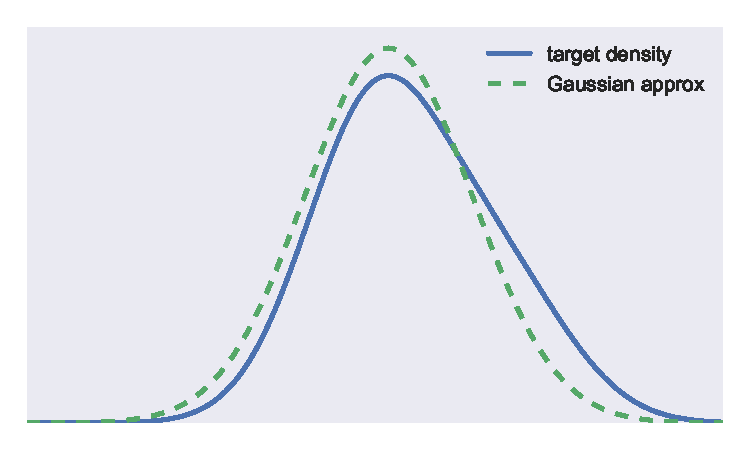
\includegraphics[width=0.9\linewidth]{fig/Laplace_approximation_comic}
\end{center}

}

\frame{
	\frametitle{Target approximation using 2nd order Taylor/Laplace (3)}
	\textbf{Advantages}
	\begin{itemize}
		\item almost as fast as finding optimal point + $O(\targdim^3)$ for matrix inversion or cholesky decomposition
		\item rather accurate in high density regions
		\item Gaussian allows many follow-up calculation in closed form
	\end{itemize}
	\textbf{Disadvantages}
	\begin{itemize}
		\item doesn't work for distributions over discrete spaces
		\item bad representation of heavy tails and rare events
		\item asymptotic  correctness not attainable (no asymptotics at play)
	\end{itemize}
	
}

\section{Ordinary Monte Carlo}

\frame{
\frametitle{Ordinary Monte Carlo}
\begin{itemize}
	\item Bayes optimal prediction for new input $\pred$ is expected $\outc$
	$$\outc_{opt} = \Expect_\targd [ \outc \, p(\outc|\pred,\Rv)] = \int \outc \, p(\outc|\pred,\Rv) \targd(\Rv) \mathrm{d} \Rv$$
	\item assume we can directly sample from distribution given by density $\targd(\Rv) = p(\Rv|\dat)$
	\item then  by the law of large numbers
	$$\outc_{opt} \approx \frac{1}{\nsamp} \sum_{i=1}^{\nsamp}  \sum_{\outc} \outc \,  p(\outc|\pred,\parsmp_i)$$ for finitely many values of $y$ and $\parsmp_i \sim \targd$ and
	 $$\outc_{opt} \approx \frac{1}{\nsamp} \sum_{i=1}^{\nsamp} \outcsmp_i$$
	for  $\outcsmp_i \sim p(\outc|\pred,\parsmp_i)$
\end{itemize}
}

\frame{
	\frametitle{Convergence rate of Monte Carlo}
	\begin{itemize}
		\item let $\outcest$ be the Monte Carlo (MC) estimate of $\outc_{opt}$
		\item MC is unbiased, i.e. $\Expect [\outcest] = \outc_{opt}$
		\item Standard deviation decreases at rate $O\left(\frac{1}{\sqrt{\nsamp}}\right)$
		\begin{align*}
		{\color{blue}\Var[\outcest]} &=\Expect\left[\left(\frac{1}{\nsamp} \sum_{i=1}^\nsamp \outcsmp_i - \Expect\left[\frac{1}{\nsamp} \sum_{i=1}^\nsamp \outcsmp_i \right]\right)^2\right] \\
		&= \frac{1}{\nsamp^2} \Var \left( \sum_{i=1}^\nsamp \outcsmp_i \right) 
		= {\color{blue}\frac{1}{\nsamp}  \Var (  \outcsmp_i )} \\
		\end{align*}
		\item unbiasedness and same rate hold for estimating $\Expect_\targd [\targfunc(\Rv)]$ for functional $\targfunc$ using Monte Carlo
	\end{itemize}
	\todo{Change to $\Rv$}
}

\frame{
\frametitle{Properties ordinary Monte Carlo}
\textbf{Advantages}
\begin{itemize}
	\item rate independent of dimension of $\Rv$, $\outc$
	\item unbiased
	\item can be applied when integral $\Expect_\targd [\targfunc(\Rv)]$ not given in closed form
\end{itemize}
\textbf{Disadvantages}
\begin{itemize}
	\item have to be able to sample from $\targd$
	\item if $\Var[\targfunc(\parsmp_i)]$ large, so is the variance of our estimator
\end{itemize}
}

\frame{
\frametitle{Importance sampling trick}
\begin{itemize}
	\item if we can't sample from $\targd$, we can still use MC
	\begin{align*}
		{\color{blue}\targInt := \Expect_\targd [\targfunc(\Rv)]} &= \int \targfunc(\Rv) \targd(\Rv) \mathrm d \Rv =  \int \targfunc(\Rv) \frac{\targd(\Rv)}{\propd(\Rv)} \propd(\Rv) \mathrm d \Rv \\
		&\approx  {\color{blue} \frac{1}{\nsamp} \sum_{i=1}^{\nsamp}\targfunc(\parsmp_i)\iw_i =: \widehat{\targInt}_\propd}
	\end{align*}
	for $\parsmp_i \sim \propd$ and $\iw_i = {\targd(\parsmp_i)}/{\propd(\parsmp_i)}$
	\item called \emph{importance sampling} (IS)
	\item assumes that $\targd(\Rv) \targfunc(\Rv) \neq 0 \Rightarrow \propd(\Rv) > 0$
	\item assumes that $\targd$ can be evaluated in normalized form
\end{itemize}
}


\frame{
\frametitle{Importance sampling variance and confidence interval}
\begin{itemize}
	\item we have $\Var[\widehat{\targInt}_\propd] = \sigma_\propd^2/\nsamp$ and can estimate
	\begin{align*}
		\sigma_\propd^2 & = \Expect[(\targfunc(\parsmp_i)\iw_i)^2] - \Expect[\targfunc(\parsmp_i)\iw_i]^2 \\
		&= \Expect[(\targfunc(\parsmp_i)\iw_i - \Expect[\targfunc(\parsmp_i)\iw_i])^2] \\
		 &\approx \sum_{i=1}^{\nsamp}[(\targfunc(\parsmp_i)\iw_i - \widehat{\targInt}_\propd)^2]
	\end{align*} 
	\item confidence interval for estimator $\widehat{\targInt}_\propd$ using gaussian cdf method
\begin{center}
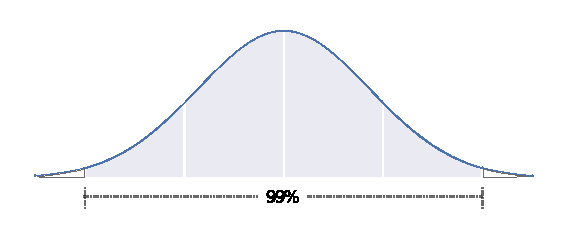
\includegraphics[width=0.7\linewidth]{fig/confidence_intervall}
\end{center}
%	\item when do we get high, when low variance?
\end{itemize}
}

\frame{
	\frametitle{Importance sampling variance minimization}
	\begin{itemize}
		\item how do we choose an optimal $\propd$?
		\item estimator always unbiased, so variance only source of error
		$$\sigma_\propd^2  = \Expect_\propd[(\targfunc(\parsmp_i)\iw_i)^2] - \Expect_\propd[\targfunc(\parsmp_i)\iw_i]^2 $$
		\item can be shown to be minimized at $$\propd(\Rv) = |\targfunc(\Rv)|\targd(\Rv)/\int|\targfunc(\Rv)|\targd(\Rv) \mathrm d \Rv$$
		\item so to get the optimal $\propd$ we need to solve the original problem (integration wrt $\targd$)!
		\item simple approach sample from Laplace approximation
		\item awful performance when proposal too narrow
	\end{itemize}
}

\frame{
\frametitle{Proposal density wider than target density}

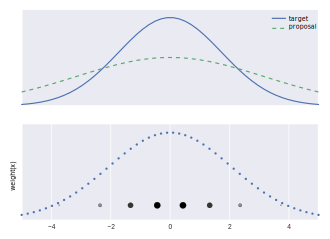
\includegraphics{fig/IS_finite_variance_comic}

}

\frame{
	\frametitle{Target density wider than proposal density}
		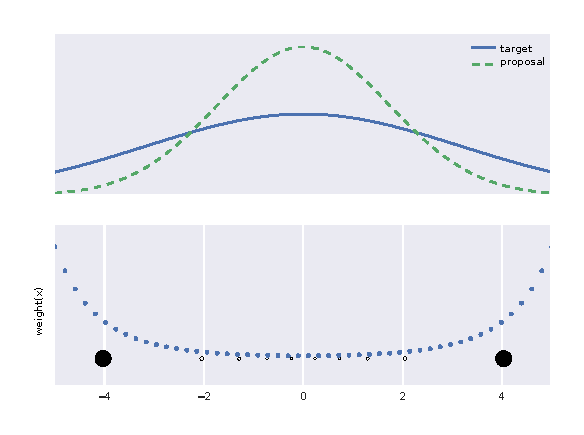
\includegraphics{fig/IS_infinite_variance_comic}
}

\frame{
\frametitle{Importance sampling variance, non-normalized case}
\begin{itemize}
	\item as a rule of thumb, IS problematic when $$\lim_{|\Rv|\to \infty} \targd(\Rv)/\propd(\Rv) \to \infty$$
	\item a common strategy is to sample from heavy-tailed distributions (i.e. not Gaussians!)
	\item in Bayesian problems, we typically can't evaluate $\targd$ in normalized form, only $\tilde{\targd}(\Rv) = p(\dat|\Rv) p(\Rv)  =  \evid \, {\targd}(\Rv)$
	\item using standard IS with $\tilde \targd$ we approximate
	$$\int \targfunc(\Rv) \frac{\tilde{\targd}(\Rv)}{\propd(\Rv)} \propd(\Rv) \mathrm d \Rv = \evid \int \targfunc(\Rv) \frac{\targd(\Rv)}{\propd(\Rv)}\propd(\Rv) \mathrm d \Rv$$
	so how do we get rid of useless (for now) $\evid$?
	
\end{itemize}
}

\frame{
	\frametitle{Self-Normalized Importance Sampling}
	\begin{itemize}
		\item in case of unnormalized $\tilde \targd$ the \emph{self-normalized Importance Sampling} estimator can be used
		\item idea is to simply estimate $\evid$ using standard IS
		$$\int \tilde \targd(\Rv) \mathrm d \Rv = \int \evid \, \targd(\Rv) \mathrm d \Rv = \int \evid \frac{ \targd(\Rv)}{\propd(\Rv)} \mathrm d \Rv \approx \frac{1}{\nsamp} \sum_{i=1}^{\nsamp} \frac{ \targd(\parsmp_i)}{\propd(\parsmp_i)} = \widehat{\evid}$$
		for $\parsmp_i \sim \propd$
		\item when taking  $\iw_i = \frac{\targd(\Rv)}{\widehat{\evid}\propd(\Rv)}$ we again get $$\targInt \approx \sum_{i=1}^{\nsamp}[\targfunc(\parsmp_i)\iw_i] =  \widehat{\targInt}_\propd$$
		\item consistent by standard results, unbiased asymptotically in $\nsamp$, often has lower variance than standard IS \citep{Robert2004}
	\end{itemize}
}

\frame{
\frametitle{Effective sample size}
\begin{itemize}
	\item quality assessment: how many i.i.d. samples from $\targd$ are our samples from $\propd$ equivalent to
	\item one common measure is \emph{effective sample size}, estimated as
	$$ \nsamp_e = \frac{(\sum_{i=1}^{\nsamp} \iw_i)^2}{\sum_{i=1}^{\nsamp} \iw_i^2} $$
	where weights are normalized to sum to $1$ $$\iw_i = \frac{\targd(\parsmp_i)/\propd(\parsmp_i)}{\sum_{i=1}^{\nsamp} \targd(\parsmp_i)/\propd(\parsmp_i)}$$
\end{itemize}	
}

\section{Population Monte Carlo}

\frame {
	\frametitle{Adaptive Importance Sampling: Population Monte Carlo}
	\begin{itemize}
		\item Population Monte Carlo \citep[PMC;][]{Cappe2004}
		\begin{itemize}
			\item improves proposal distributions $\propd_{t}$ over iterations indexed by $t$ by adapting to samples from previous iterations
			\item resulting estimate is consistent by the law of large numbers 
			\begin{align*}
			\targInt =	\int \targfunc(\Rv) \targd(\Rv) \textrm{d}\Rv & = \int \targfunc(\Rv) \frac{\targd(\Rv)}{\propd(\Rv)} \propd(\Rv) \textrm{d}\Rv\\
			& = \iint \targfunc(\Rv) \frac{\targd(\Rv)}{\propd_t(\Rv)} \propd_t(\Rv) \textrm{d}\Rv~g(\propd_t)\textrm{d}\propd_t
			\end{align*}
			\item $g$ is any distribution on the $\propd_t$, so can adapt in any way we like
			\item simple special case of Sequential Monte Carlo
		\end{itemize}
	\end{itemize}
}

\frame {
	\frametitle{Population Monte Carlo \cite{Cappe2004}}
	\begin{algorithmic}
		\STATE {\bfseries Input:} initial proposal density $\propd_0$, unnormalized density $\tilde \targd $, population size $p$, sample size $m$
		\STATE {\bfseries Output:} lists $P,W$ of $m$ samples and weights
		
		
		\STATE Initialize $\parsmp = List()$
		\STATE Initialize $W = List()$
		\WHILE{$len(\parsmp) \leq \nsamp$}
		\STATE construct proposal distribution $\propd_{t}$
		\STATE generate  set of $p$ samples $\SaS_t$ from $\propd_{t}$ and append it to $\parsmp$
		\STATE ~~~for all $\smp \in \SaS_t$ append weights $\tilde\targd(\smp)/\propd_{t}(\smp)$ to $W$
		
		\ENDWHILE
	\end{algorithmic}
}

\frame{
	\frametitle{PMC properties}
	\begin{itemize}
		\item proposals $\propd_{t}$ must not degenerate to distributions that are `too thin compared to $\targd $ 
		\item diminishing adaptation not a requirement, unlike in adaptive MCMC  (which we will see)
		\item can adapt any which way we like without need to proof ergodicity
		\item probability of model given the data at any time for model choice and Bayesian testing (this is $\evid$!)
		\item using randomized Low Discrepancy point sets, we can improve convergence rates more easily than in Metropolis-Hastings
	\end{itemize}
}

\frame{
	\frametitle{Random-Walk PMC (1)}
	\begin{itemize}
		\item pick some $\propd_0$, for example some Gaussian or Student-$t$ distribution
		\item given samples $\parsmp_{t-1,i}$ from iteration $t-1$, choose as next proposal the mixture of Gaussians
		$$\propd_t = \sum_{i=1}^{p}\DNorm(\parsmp_{t-1,i}, M)$$
		for fixed covariance matrix M
		\item iterate for desired number of iterations
	\end{itemize}
}

\frame{
	\frametitle{Random-Walk PMC (2)}
	
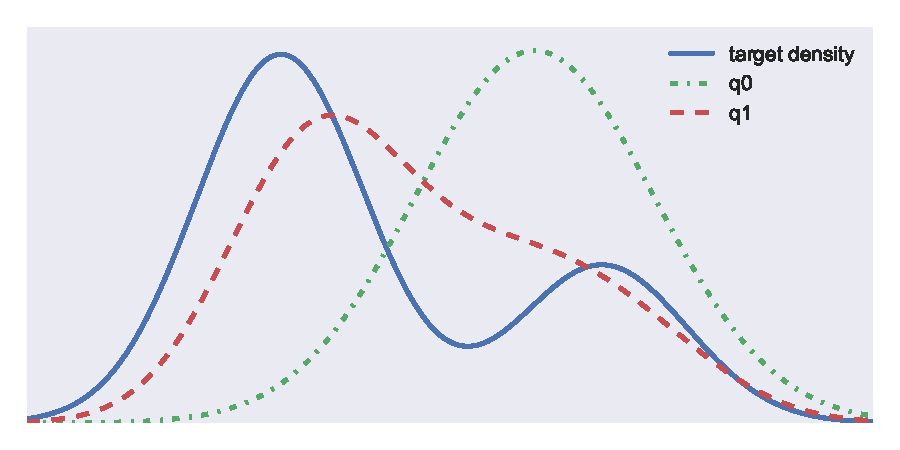
\includegraphics[width=\linewidth]{fig/PMC_rw_comic}

}

\frame{
	\frametitle{PMC properties}
	\textbf{Advantages}
	\begin{itemize}		
		\item simple to understand
		\item often performs better empirically than Metropolis-Hastings with same proposal distribution (next lecture)
	\end{itemize}
	\textbf{Disadvantages}
	\begin{itemize}		
		\item Central Limit Theorems only for special cases
		\item not as widely used as Metropolis-Hastings
		\item not  as well understood as Metropolis-Hastings and MCMC in general
	\end{itemize}
}
\frame{
	\frametitle{What have we seen?}
	\begin{itemize}
		\item Why we need posterior distributions rather than point estimates (Bayes optimality)
		\item Laplace approximation as computationally cheap posterior approximation
		\item ordinary Monte Carlo and convergence rate $O(1/\sqrt{\nsamp})$
		\item importance sampling
		\begin{itemize}
			\item standard case: use MC when we cant sample from target
			\item self-normalized case: when target density is not normalized
			\item adaptive schemes: Population Monte Carlo
		\end{itemize}
	\end{itemize}
}

\section{Markov Chain Monte Carlo}


\frame{
\frametitle{Sampling by constructing a Markov process}
\begin{itemize}
	\item we might sample from arbitrary density $\targd$ by constructing Markov process that has $\targd$ as 'invariant' distribution
	\item i.e. start with some point $\parsmp_0$, generate point $\parsmp_1$ from constructed Markov process
	\item if process has invariant distribution $\targd$, then 
	$$\parsmp_0 \sim \targd \Rightarrow \parsmp_1 \sim \targd$$
	\item some constructions guarantee $\parsmp_t \sim \targd$ for some $t\in \Nats$, no matter what the distribution of $\parsmp_0$ is
	\item these methods are called \emph{Markov Chain Monte Carlo} (MCMC)
\end{itemize}
}

\frame{
	\frametitle{Detailed balance}
	\begin{itemize}
		\item denote transition probability from current state $\Rv$ to new state $\Rv'$ by $\MK(\Rv'|\Rv)$
		$$\Rv \rightarrow_{\MK(\cdot|\Rv)} \Rv'$$
		\item one way of constructing a Markov chain leaving some $\targd$ invariant is to satisfy detailed balance wrt $\targd$
		$$ \targd(\Rv)\MK(\Rv'|\Rv) = \targd(\Rv')\MK(\Rv|\Rv') $$
		\emph{Proof of invariance (sketch)}:  
		\begin{align*}
		\int \targd(\Rv)\MK(\Rv'|\Rv) \mathrm d \Rv & = \int \targd(\Rv')\MK(\Rv|\Rv') \mathrm d \Rv  \\
		 & = \targd(\Rv')  \underbrace{\int \MK(\Rv|\Rv') \mathrm d \Rv}_{=1} \\
		 & = \targd(\Rv')  &
		\end{align*}
	\end{itemize}
}

\frame{
	\frametitle{Metropolis-Hastings construction}
	\begin{itemize}
		\item idea: construct algorithm that satisfies detailed balance
		\item use two parts
		\begin{itemize}
			\item a distribution for proposing a move $\propd(\cdot|\Rv)$
			\item probability for accepting proposed move $\acc(\cdot|\Rv)$ (else stay at current state)
		\end{itemize}
		\item Algorithm
		\begin{itemize}
			\item at state $\Rv$, draw sample $\Rv' \sim \propd(\cdot|\Rv)$
			\item with probability $\acc(\Rv'|\Rv)$, new chain state is $\Rv'$, else $\Rv$
		\end{itemize}
	\end{itemize}
}

\frame{
	\frametitle{MH Markov kernels}
	\begin{itemize}
		\item at state $\Rv$, draw sample $\Rv' \sim \propd(\cdot|\Rv)$
		\item with probability $\acc(\Rv'|\Rv)$, new chain state is $\Rv'$, else $\Rv$
	
	\begin{align*}
	 \MK(\Rv'|\Rv) & = \propd(\Rv'|\Rv)\acc(\Rv'|\Rv) \\
	 \MK(\Rv|\Rv)  & = \propd(\Rv|\Rv)+\int \propd(\Rv'|\Rv)(1-\acc(\Rv'|\Rv)) \mathrm d \Rv'
	\end{align*}
		\item if $\propd$ is fixed we need to find $\acc$ such that detailed balance holds
	\end{itemize}
}

\frame{
	\frametitle{MH acceptance probability}
	\begin{itemize}
		\item Algorithm
		\begin{itemize}
			\item at state $\Rv$, draw sample $\Rv' \sim \propd(\cdot|\Rv)$
			\item with probability $\acc(\Rv'|\Rv)$, new chain state is $\Rv'$, else $\Rv$
		\end{itemize}
		\item from detailed balance for $\Rv \neq \Rv'$
		\begin{align*}
		 \targd(\Rv)\MK(\Rv'|\Rv) &= \targd(\Rv')\MK(\Rv|\Rv') & \Leftrightarrow\\
		\targd(\Rv)\propd(\Rv'|\Rv)\acc(\Rv'|\Rv) &= \targd(\Rv')\propd(\Rv|\Rv')\acc(\Rv|\Rv') & \Leftrightarrow\\
		\frac{\acc(\Rv'|\Rv)}{\acc(\Rv|\Rv')} &= \frac{\targd(\Rv')\propd(\Rv|\Rv')}{\targd(\Rv)\propd(\Rv'|\Rv)} &
		\end{align*}
		\item this equality holds for the choice
		$$  \acc(\Rv'|\Rv) = \min\left(1, \frac{\targd(\Rv')\propd(\Rv|\Rv')}{\targd(\Rv)\propd(\Rv'|\Rv)}\right) $$
	\end{itemize}
}

\frame{
\frametitle{MH acceptance probability choice and detailed balance}
Pick
$ \acc(\Rv'|\Rv) = \min\left(1, r \right) $
for
$ r := \frac{\targd(\Rv')\propd(\Rv|\Rv')}{\targd(\Rv)\propd(\Rv'|\Rv)}$.\\
Then detailed balance holds if
$$\frac{\acc(\Rv'|\Rv)}{\acc(\Rv|\Rv')} = r$$
case $r < 1$:
$$\frac{\acc(\Rv'|\Rv)}{\acc(\Rv|\Rv')} = \frac{\min\left(1, r \right)}{\min\left(1, 1/r \right)} = \frac{r}{1} = r$$
case $r \geq 1$:
$$\frac{\acc(\Rv'|\Rv)}{\acc(\Rv|\Rv')} = \frac{\min\left(1, r \right)}{\min\left(1, 1/r \right)} = \frac{1}{1/r} = r$$
}

\frame{
\frametitle{Average acceptance probabilities}
\begin{figure}
\centering
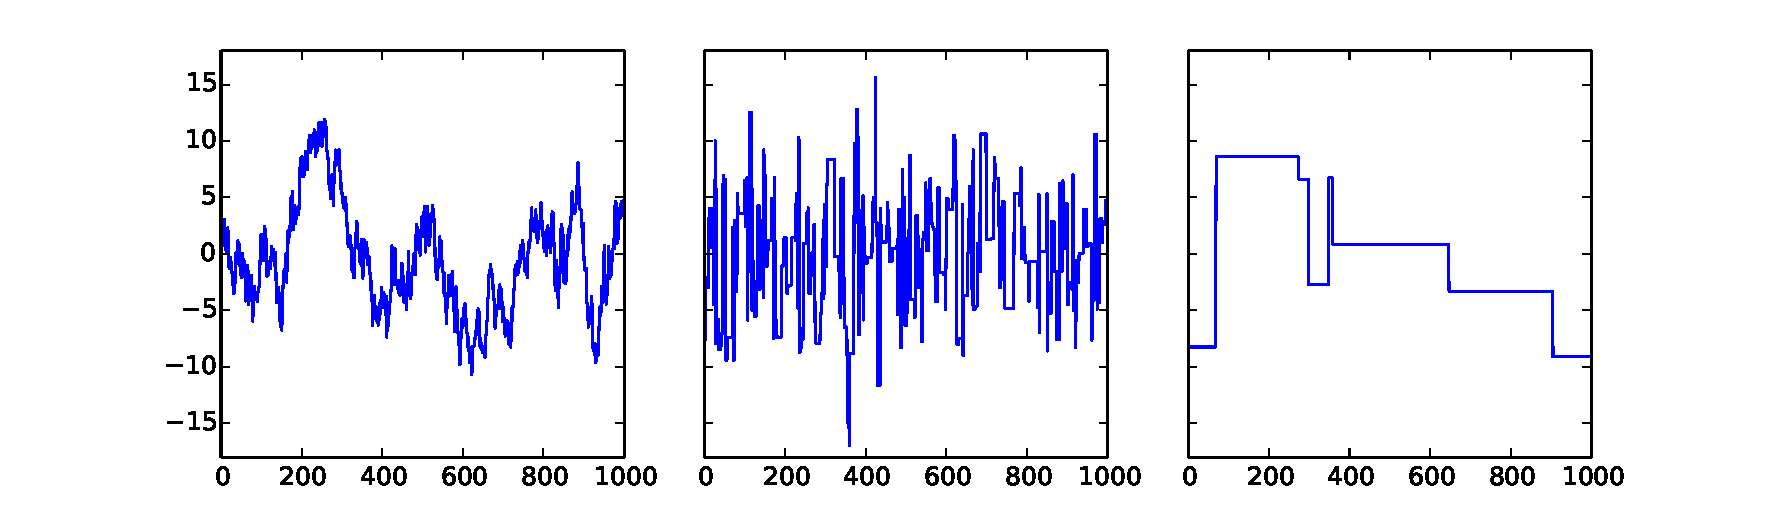
\includegraphics[width=\linewidth]{fig/Acceptance_rates_high_to_low}
\caption{Average acceptance close to $1$ (left, highly correlated) close to $0.5$ (middle) and close to $0$ (right, highly correlated)}
\label{fig:Acceptance_rates_high_to_low}
\end{figure}

}

\frame{
	\frametitle{Choice of proposal (1)}
	\begin{itemize}
		\item must ensure reversibility
		$$ \propd(\Rv'|\Rv) > 0\Rightarrow \propd(\Rv|\Rv') > 0$$
		\item opposing goals
		\begin{itemize}
			\item $\propd$ should be broad to quickly cover all the space
			\item but then many proposed points will be rejected because of low value under $\targd$
		\end{itemize}
		
	\end{itemize}
	
\begin{center}
	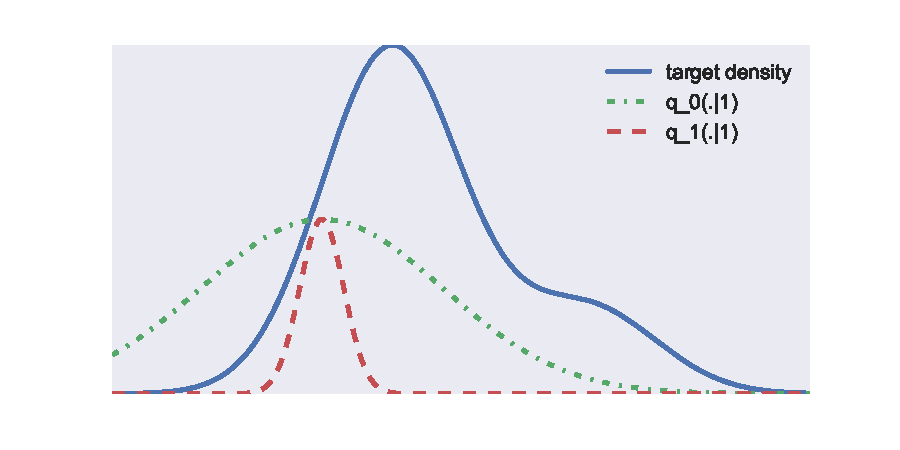
\includegraphics[width=0.7\linewidth]{fig/MH_rw_comic}\\
	$\acc(\Rv'|\Rv) = \min\left(1, {\targd(\Rv')\propd(\Rv|\Rv')}/{\targd(\Rv)\propd(\Rv'|\Rv)}\right)$
\end{center}
	}

\frame{
	\frametitle{Choice of proposal (2)}
	\begin{itemize}
		\item if all moves are accepted, we probably propose very small steps
		\item if all moves are rejected, steps are very large (proposal variance high)
		\item intuitively, average acceptance probability shouldn't be close to $0$ or to $1$, rather in between
		\item under strong conditions on target $\targd$, optimal acceptace rates for certain $\propd$ have been derived
		\begin{itemize}
			\item $\propd(\cdot|\Rv) = \DNorm(\cdot; \Rv, \sigma^2 M)$: $\acc_{opt} \approx 0.234$ for dimensionality $>5$
			\item $\propd(\cdot|\Rv) = \DNorm(\cdot; \Rv + \lambda \nabla \log \targd(\Rv), \sigma^2 M)$: $\acc_{opt} \approx 0.56$
			\item \dots
		\end{itemize}
		\item ideal: find parameters $\lambda, M, \sigma^2$ s.t. we attain optimal average acceptance rate
	\end{itemize}
}

\frame{
	\frametitle{Optimal proposal (1)}
\begin{figure}
\centering
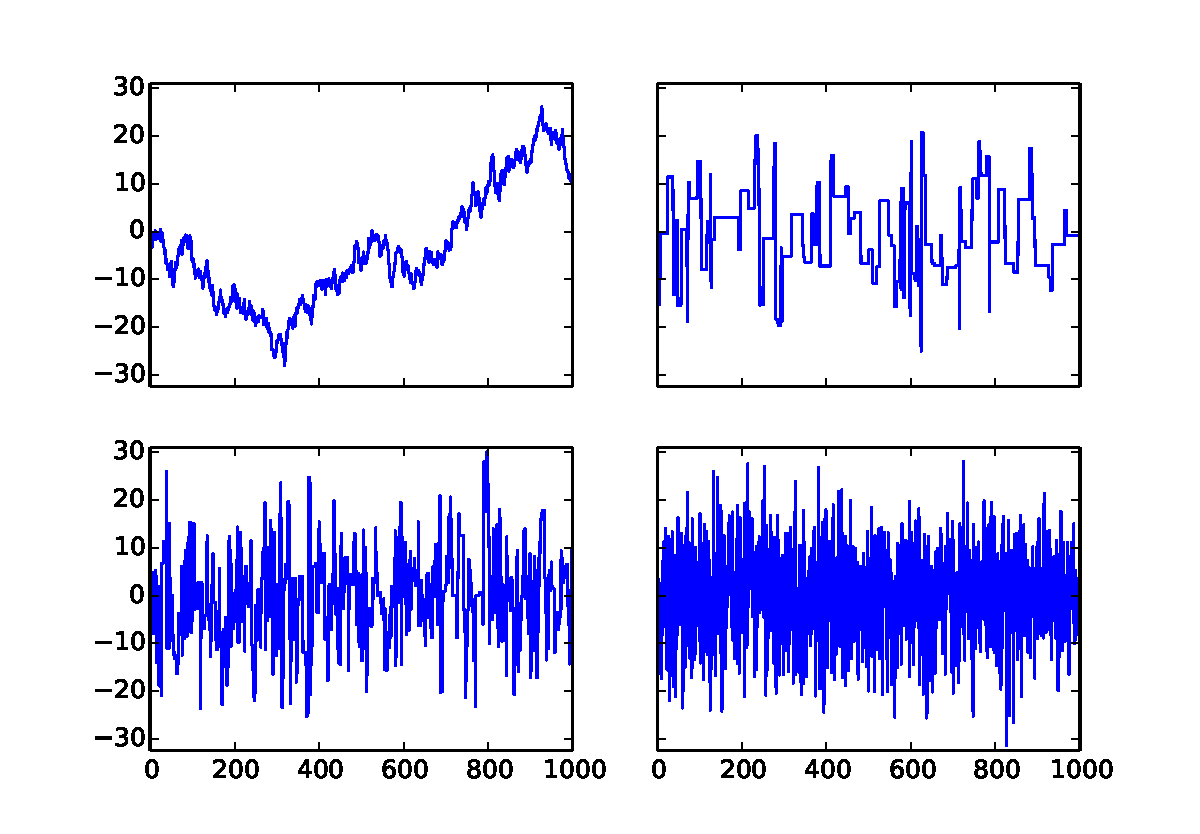
\includegraphics[width=0.7\linewidth]{fig/Acceptance_rates_high_low_optimal_iid}
\caption{\emph{Top}: Too high high (left, $0.96$) and too low (right, $0.13$) acceptance rates.
	\emph{Bottom}: approx. optimal rate for 1D target (left, $0.47$), i.i.d. target samples (right).
	}
\label{fig:Acceptance_rates_high_low_optimal_iid}
\end{figure}

}

\frame{
	\frametitle{Optimal proposal (2)}
	\begin{itemize}
		\item assume we have a single scaling parameter as in $\propd(\cdot|\Rv) = \DNorm(\cdot; \Rv, \sigma^2 M)$
		\item increasing $\sigma^2$ decreases average acceptance rate and vice versa
		\item naive tuning
		\begin{itemize}
			\item run chains at different values for $\sigma^2$
			\item compute average acceptance rate
			\item iterate until good value found
		\end{itemize}
		\item all asymptotic arguments from Markov chain theory still hold
		\item computationally costly
	\end{itemize}
}

\frame{
	\frametitle{Optimal proposal (3)}
	
	
	}

\section{Conclusion}
\frame{
\frametitle{Conclusion (1)}
\begin{itemize}
	\item 
\end{itemize}
}


\frame{
\centerline{\LARGE \emph{Thanks!}}
}

\AtBeginSection{}
\frame[allowframebreaks]{
\frametitle{Literature}
\bibliographystyle{apalike}
\bibliography{library}
}
\end{document}
